\documentclass[../main.tex]{subfiles}

\begin{document}

\chapter{Model Development}
\label{cha:model}

\begin{modelchapter}

The following chapter details the process to develop a model for the sensation
of fluctuation strength, based on \citeauthor{daniel1997psychoacoustical}'s
roughness model~\cite{daniel1997psychoacoustical}. The model will be analyzed in
stages, where the changes needed to adapt it to this particular case will be
detailed. After that, a procedure to adjust the parameters of the model is
presented. Finally, the results of the fluctuation strength model will be
presented, and the limitations of the data fitting will be addressed.

\section{Roughness Model}

\citeauthor{daniel1997psychoacoustical}'s roughness model
\cite{daniel1997psychoacoustical}will be used as a basis for a fluctuation
strength model adapted to the data obtained in the experimental stage of this
study. It has already been mentioned in \Cref{cha:theoretical} that roughness
and fluctuation strength sensations are similar from a physical point of view;
both attributes arise from modulated sounds. As such, the methodology used to
model the roughness sensation might be adequate to also model the fluctuation
strength sensation.

The structure of the roughness model is presented in \Cref{fig:roughness_model}.
The model can be separated into three stages:
\begin{enumerate}
  \item Peripheral stage
  \item Modulation depth extraction stage
  \item Specific roughness stage
\end{enumerate}

\begin{figure}[!ht]
  \centering
  \resizebox{!}{15cm}{\begin{tikzpicture}
  [node distance=1cm,
  start chain=going below]

  \node[blockbig, join](input)
    {input signal};
  \node[blockbig, join](window)
    {200 ms frame of the sampled input signal\\%
    weighted with a Blackman window};
  \node[blockbig, join](patterns)
    {transformation of the frame spectrum\\into excitation patterns};
  \node[blockbig, join](filterbank)
    {critical-band filterbank of 47 overlapping channels\\%
    at $z_i = 0.5\ i$ Bark and a bandwidth $\Delta z = 1$ Bark};
  \node[blockmedium, join](fourier)
    {$e_{i}(t)\to|e_{i}(t)|\to\mathcal{F}(|e_{i}(t)|)$};
  \node[blocksmall, below left=1cm and -41.5mm of fourier](dc)
    {DC: $h_{0,i}=\overline{|e_{i}(t)|}$};
  \node[blocksmall, below right=1cm and -41.5mm of fourier](filter)
    {bandpass filtering:\\ $\mathcal{F}(|e_{i}(t)|) \cdot H_{i}(f_{mod})$};
  \node[blocksmall, below=3cm of fourier](m*)
    {${m_i}^* = \tilde{h}_{BP,i}(t)/h_{0,i}$};
  \node[blocktiny, below left=1cm and 15mm of m*](correlation_left)
    {correlation};
  \node[blocktiny, below right=1cm and 15mm of m*](correlation_right)
    {correlation};
  \node[blockmediumsmall, below=3cm of m*](ri)
    {$r_i = \big(g(z_i) \cdot {m_i}^* \cdot k_{i-2} \cdot k_i \big)^2$};
  \node[circle, draw=black, very thick, on chain](sum){+};
  \node[on chain](R){R};

  \node[below left=2mm and -5.75cm of filterbank](i){i};
  \node[below left=2mm and -1cm of filterbank](k1){1};
  \node[below left=2mm and -1.75cm of filterbank](d1){$\cdots$};
  \node[below right=2mm and -1.25cm of filterbank](k47){47};
  \node[below right=2mm and -2cm of filterbank](d2){$\cdots$};

  \node[below right=-8mm and 1cm of m*](hbpi){$h_{BP,i}(t)$};
  \node[below left=0cm and 1.5cm of m*](ic2){i};
  \node[below left=0cm and 2.75cm of m*](i-2){i$-$2};
  \node[below right=0cm and 1.5cm of m*](ic1){i};
  \node[below right=0cm and 2.75cm of m*](i+2){i+2};
  \node[below left=5mm and -10mm of correlation_left](ki-2){$k_{i-2}$};
  \node[below right=5mm and -10mm of correlation_right](ki){$k_i$};

  \node[left=4.5cm of sum](c1){1};
  \node[right=4.5cm of sum](c47){47};

  \draw[line] (filterbank.south) +(-5.5,0.0) -- +(-5.5,-0.5);
  \draw[line,dotted] (filterbank.south) +(-5.5,-0.5) -- +(-5.5,-1.0);
  \draw[line] (filterbank.south) +(5.5,0.0) -- +(5.5,-0.5);
  \draw[line,dotted] (filterbank.south) +(5.5,-0.5) -- +(5.5,-1.0);

  \draw[line] (dc.north)--(dc|-fourier.south);
  \draw[line] (filter.north)--(filter|-fourier.south);
  \draw[line] (dc.south) -- +(0.0,-1.4) -- (m*.west);
  \draw[line] (filter.south) -- +(0.0,-2.45);
  \draw[line] (m*.east) -- +(0.8,0.0);
  \draw[line] (m*.south) -- (ri.north);
  \draw[arrow] (m*.south) -- +(0.0,-0.5) -- +(-4.5,-0.5) -- +(-4.5,-1.0);
  \draw[arrow] (m*.south) -- +(0.0,-0.5) -- +(4.5,-0.5) -- +(4.5,-1.0);
  \draw[arrow] (ri.south) -- (sum.north);
  \draw[arrow] (correlation_left.south) -- +(0.0,-1.4) -- (ri.west);
  \draw[arrow] (correlation_right.south) -- +(0.0,-1.4) -- (ri.east);
  \draw[arrow] (sum.south) -- (R.north);

  \draw[line,dashed] (sum.west) +(-5.0,1.0) -- +(-4.5,0.5);
  \draw[arrow] (sum.west) +(-4.5,0.5) -- +(-4.0,0.0) -- (sum.west);
  \draw[line,dashed] (sum.east) +(5.0,1.0) -- +(4.5,0.5);
  \draw[arrow] (sum.east) +(4.5,0.5) -- +(4.0,0.0) -- (sum.east);

  \draw[arrow] (correlation_left.north) +(-0.5,0.5) -- +(-0.1,0.5) --
    +(-0.1,0.0);
  \draw[line,dashed] (correlation_left.north) +(-1.0,0.5) -- +(-0.5,0.5);
  \draw[arrow] (correlation_right.north) +(0.5,0.5) -- +(0.1,0.5) --
    +(0.1,0.0);
  \draw[line,dashed] (correlation_right.north) +(1.0,0.5) -- +(0.5,0.5);

  \draw[arrow,dashed] (sum) +(-1.0,1.0) -- +(-0.25,0.25);
  \draw[arrow,dashed] (sum) +(1.0,1.0) -- +(0.25,0.25);

  \filldraw[black] (m*.east) +(0.8,0.0) circle (2pt);
  \filldraw[black] (filter.south) +(0.0,-2.5) circle (2pt);

\end{tikzpicture}
}
  \caption%
    {Structure of roughness model~\cite[pp.~116]{daniel1997psychoacoustical}}
\label{fig:roughness_model}
\end{figure}

\subsection{Peripheral Stage}

First, the input signal is divided into frames, which in the original roughness
model have a 200~ms duration. For the fluctuations strength case this must be
increased, in order to achieve higher frequency resolution to be able to process
stimuli with frequency components with little separation among them (e.g.,
$f_m = 4$~Hz). This can be achieved by manipulating two variables, namely the
sampling frequency and the number of samples. For this study it has been decided
to keep the sampling frequency at 44.1~kHz, the most common frequency used in
audio recordings. The number of samples is chosen such that it contains at least
three periods of the slowest modulation envelope, following the criteria
presented by~\textcite[pp.~97]{Boersma1993}. The slowest stimulus has a
modulation frequency of 0.25~Hz, thus three periods would constitute a 12~s
frame duration. This results in a number of samples of 1048576 ($2^{20}$) and a
duration of 23.77~s, using the closest value that is a power of 2.

After the frame separation, a Blackman window is applied to the frame to reduce
spectral leakage. Following this, the outer and middle ear transmission effects
are taken into account by transforming the frame into the frequency domain, and
multiplying its components by the parameter $a_0$, shown in \Cref{fig:a0}.

\begin{figure}[!ht]
  \centering
  \includegraphics[height=8cm]{a0}
  \caption{Outer and middle ear transmission effects parameter $a_0$}
\label{fig:a0}
\end{figure}

After this, the input frame spectrum is transformed into excitation patterns
using \citeauthor{Terhardt1979}'s approach \cite{Terhardt1979}. This method is a
non-linear one, where the lower and upper slopes of the excitation patterns
differ. The lower slopes are independent of the stimulus center frequency, and
are defined by:
\begin{equation}
  S_1 = -27 \quad \frac{\text{dB}}{\text{Bark}}
  \label{eq:lower_slopes}
\end{equation}

The upper slopes depend on the center frequency of the stimulus, and are defined
by the following equation:
\begin{equation}
  S_2 = [-24-\frac{0.23 \text{ kHz}}{f}+\frac{0.2 \text{ L}}{\text{dB}}]
  \quad
  \frac{\text{dB}}{\text{Bark}}
\end{equation}

After generating each of the excitation patterns for all the frequency
components, the contribution of all of these patterns is analyzed per
critical-band. The excitation patterns are processed using a critical-band
filter with 47 channels, each on them separated by 0.5 Bark and having a
bandwidth of 1 Bark.

For each critical-band, all the frequency components of the input signal are
used. Three posibles cases are defined for a given frequency component and a
critical-band. \Cref{fig:schrader} presents an example that illustrates these
three cases for a critical-band centered at 12 Bark. First, if the frequency
component falls within the critical-band, then the frequency component is not
affected in any way, i.e., is multiplied by 1. This would be the case of
frequency component (2) in \Cref{fig:schrader}. If the frequency component is
above the critical-band, then the value of the excitation pattern that
corresponds to $z_i + 0.5$, $z_i$ being the Bark value of the center frequency
of the current critical-band (12 in the example), is used to multiply the
frequency component that produces this excitation pattern. This would be the
case for frequency component labeled (3) in \Cref{fig:schrader}. If the
frequency component is below the critical-band, then the $z_i - 0.5$ value is
used; frequency component (1) in \Cref{fig:schrader}.

\begin{figure}[!ht]
  \centering
  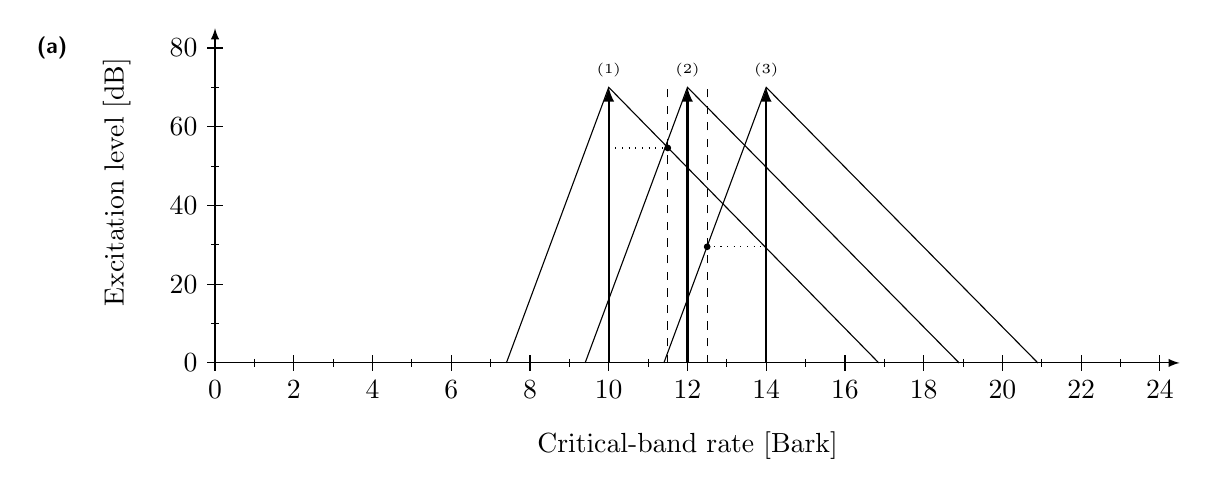
\begin{tikzpicture}
  % axis
  \draw[-latex] (-0.1,0) -- (12.25,0);
  \draw[-latex] (0,-0.1) -- (0,4.25);

  % ticks
  \foreach \x in {0.5,1.5,2.5,3.5,4.5,5.5,6.5,7.5,8.5,9.5,10.5,11.5}
    \draw[shift={(\x,0)}] (0,0.05) -- (0,-0.05);
  \foreach \x/\xtext in {0/0,1/2,2/4,3/6,4/8,5/10,6/12,7/14,8/16,9/18,10/20,11/22,12/24}
    \draw[shift={(\x,0)}] (0,0.1) -- (0,-0.1) node[below] {$\xtext$};

  \foreach \y in {0.5,1.5,2.5,3.5}
    \draw[shift={(0,\y)}] (0.05,0) -- (-0.05,0);
  \foreach \y/\ytext in {0/0,1/20,2/40,3/60,4/80}
    \draw[shift={(0,\y)}] (0.1,0) -- (-0.1,0) node[left] {$\ytext$};

  \draw (3.7,0) -- (5,3.5) -- (8.43,0);
  \draw (4.7,0) -- (6,3.5) -- (9.45,0);
  \draw (5.7,0) -- (7,3.5) -- (10.45,0);

  \draw[thick,-latex] (5,0) -- (5,3.5) node[above] {\tiny(1)};
  \draw[thick,-latex] (6,0) -- (6,3.5) node[above] {\tiny(2)};
  \draw[thick,-latex] (7,0) -- (7,3.5) node[above] {\tiny(3)};

  \draw[dashed] (5.75,0) -- (5.75,3.5);
  \draw[dashed] (6.25,0) -- (6.25,3.5);

  \draw[dotted] (5,2.73) -- (5.75,2.73);
  \draw[dotted] (6.25,1.475) -- (7,1.475);

  \filldraw[black] (5.75,2.73) circle (1pt);
  \filldraw[black] (6.25,1.475) circle (1pt);

  \draw (6,-0.75) node[below] {Critical-band rate [Bark]};
  \draw (-1.25,4) node[left, rotate=90] {Excitation level [dB]};

  \draw (-1.75,4) node[left] {{\sffamily \bfseries \footnotesize (a)}};

\end{tikzpicture}

  \begin{tikzpicture}
  % axis
  \draw[-latex] (-0.1,0) -- (12.25,0);
  \draw[-latex] (0,-0.1) -- (0,4.25);

  % ticks
  \foreach \x in {0.5,1.5,2.5,3.5,4.5,5.5,6.5,7.5,8.5,9.5,10.5,11.5}
    \draw[shift={(\x,0)}] (0,0.05) -- (0,-0.05);
  \foreach \x/\xtext in {0/0,1/2,2/4,3/6,4/8,5/10,6/12,7/14,8/16,9/18,10/20,11/22,12/24}
    \draw[shift={(\x,0)}] (0,0.1) -- (0,-0.1) node[below] {$\xtext$};

  \foreach \y in {0.5,1.5,2.5,3.5}
    \draw[shift={(0,\y)}] (0.05,0) -- (-0.05,0);
  \foreach \y/\ytext in {0/0,1/20,2/40,3/60,4/80}
    \draw[shift={(0,\y)}] (0.1,0) -- (-0.1,0) node[left] {$\ytext$};

  \draw[thick,-latex] (5,0) -- (5,2.73) node[above] {\tiny(1)};
  \draw[thick,-latex] (6,0) -- (6,3.5) node[above] {\tiny(2)};
  \draw[thick,-latex] (7,0) -- (7,1.475) node[above] {\tiny(3)};

  \draw (6,-0.75) node[below] {Critical-band rate [Bark]};
  \draw (-1.25,4) node[left, rotate=90] {Excitation level [dB]};

  \draw (-1.75,4) node[left] {{\sffamily \bfseries \footnotesize (b)}};

\end{tikzpicture}

  \caption{Excitation patterns and specific excitation levels for a
    critical-band channel centered at 12 Bark with 1 Bark bandwith.Three pure
    tones are presented with sound pressure levels of 70 dB and center
    frequencies of 10 Bark (1), 12 Bark (2) and 14 Bark (3). Panel (a) shows the
    original excitation patterns and specific excitation level. The dashed lines
    show the bandwidth of critical-band at 12 Bark. The dotted lines show the
    projection of the values of the tones outside the critical-band. Panel (b)
    shows the modified specific excitation levels after adjustment using the
    projected values shown in panel (a)}
\label{fig:schrader}
\end{figure}

After doing all the calculations for all the frequency components, then the real
part of an \gls{IFFT} is taken from the resulting array of the modified
frequency components, yielding this the time-varying excitation per band.

\subsection{Modulation Depth Extraction Stage}

This stage's objective is to come up with an approximation of the modulation
depth present in the incoming frame on a channel basis. For each channel signal
$e_{i}(t)$ its absolute value is obtained and its mean is then calculated with
\Cref{eq:h0i},

\begin{equation}
  h_{0,i} = \overline{|e_{i}(t)|}.
  \label{eq:h0i}
\end{equation}

The mean is then subtracted from each signal and the resulting signal is
filtered using a bandpass filter $H[f_{mod}]$, shown in \Cref{eq:hBPi},

\begin{equation}
  h_{BP,i}(t) = (e_{i}^{\prime} * H[f_{mod}])(t)
  \label{eq:hBPi}
\end{equation}
where
\begin{equation}
  e_{i}^{\prime} = |e_{i}(t)| - h_{0,i}.
\end{equation}

Finally, the modulation depth per channel is obtained by the ratio of the
\gls{RMS} value of the bandpass filtered signal and its mean, shown in
\Cref{eq:mi*},
\begin{equation}
  {m_i}^* = \tilde{h}_{BP,i}(t)/h_{0,i}.
  \label{eq:mi*}
\end{equation}

Two changes are introduced in this stage to adapt the model behavior to the
fluctuation strength scenario. First, an unique filter is used for all the 47
channels, whereas in the roughness model a different filter is used for each
channel, to take into account possible effects of the center frequency on the
modulation frequency dependency. Second, since the bandpass filter response
defines the modulation depth dependency, by adjusting it a better fit for the
fluctuation strength case can be achieved

On an implementation note with regard to the bandpass filter, the filtering is
done using a Butterworth \gls{IIR} filter. Its parameters are detailed in
\Cref{tab:bandpass_filter}.

\begin{table}[!ht]
  \centering
  \begin{tabu} to \linewidth{XX}
    \toprule
    \rowfont\bfseries
    Parameter & Value \\
    \midrule
    Stopband Frequency 1 & 0.5 [Hz] \\
    Passband Frequency 1 & 2 [Hz] \\
    Passband Frequency 2 & 8 [Hz] \\
    Stopband Frequency 2 & 32 [Hz] \\
    Stopband Attenuation 1 & 100 [dB] \\
    Passband Ripple & 3 [dB] \\
    Stopband Attenuation 2 & 100 [dB] \\
    \bottomrule
  \end{tabu}
  \caption{Bandpass filter characteristics}
\label{tab:bandpass_filter}
\end{table}

\subsection{Specific Roughness Stage}

The last stage of the model deals with the specific roughness calculation. The
model is based on the dependence of roughness on modulation depth, portrayed
by \Cref{eq:roughness_modulation_depth}.

\begin{equation}
  R \sim m^p
  \label{eq:roughness_modulation_depth}
\end{equation}

For each channel, a specific value of roughness is obtained by using the
\Cref{eq:ri}.

\begin{equation}
  r_i = [g(z_i) \cdot {m_i}^* \cdot k_{i-2} \cdot k_i]^2
  \label{eq:ri}
\end{equation}

The parameter $g(z_i)$ corresponds to a weight associated to each channel, and
it models the dependence of roughness on the center frequency of the stimulus.
Additionally, cross correlations between the two neighboring channels are
included ($k_{i-2}, k_i$) to account for phase shifts between the channels
signals. The total roughness is then obtained by summing all the specific
values for each channel, shown in \Cref{eq:total_roughness}

\begin{equation}
  R = \text{cal} \cdot \displaystyle\sum_{i=1}^{47} r_i
  \label{eq:total_roughness}
\end{equation}
where cal is a calibration constant.

In order to accommodate for the fluctuation strength scenario, a different
equation for the specific fluctuation values was proposed, that provided more
flexibility to adapt the model response to the obtained data. First, the three
factors used in the specific value calculation where assigned a separate power
coefficient to each of them, shown in \Cref{eq:fi}. In this way, the
contribution of these components can be weighted and adjusted individually.

\begin{equation}
  f_i = \big(g(z_i)\big)^{p_g} \cdot ({m_i}^*)^{p_m}
    \cdot (k_{i-2} \cdot k_i)^{p_k}
  \label{eq:fi}
\end{equation}

After the adjustments, the parameter $g(z_i)$ was removed, since the data
gathered did not show a dependence on the center frequency. Furthermore, to
avoid imaginary values when using power coefficients smaller than 1, the
absolute value of the product of the cross correlations coefficients was used.
Although this negates the subtraction of specific fluctuation due to a negative
coefficient, it yields better fitting results. The final form of the specific
fluctuation strength equation is shown in \Cref{eq:fi_final}.

\begin{equation}
  f_i = ({m_i}^{*\prime})^{0.25} \cdot |k_{i-2} \cdot k_i|^{0.375}
  \label{eq:fi_final}
\end{equation}

where

\begin{align}
  {m_i}^{*\prime} &= H({m_i}^{*\prime\prime}) \cdot {m_i}^{*\prime\prime}
  \label{eq:md_transformation_1} \\
  {m_i}^{*\prime\prime} &= {m_i}^* - 0.1
  \label{eq:md_transformation_2}
\end{align}

being $H$ the Heaviside step function.

The total fluctuation strength is then obtained using
\Cref{eq:total_fluctuation}.

\begin{equation}
  F = 0.15 \cdot \displaystyle\sum_{i=1}^{47} f_i
  \label{eq:total_fluctuation}
\end{equation}

\section{Procedure}

The parameters were adjusted using the following order:
\begin{enumerate}
  \item $p_m$
  \item $p_k$
  \item cal
  \item $H(f_{mod})$
\end{enumerate}

The order is such that the first parameter is the one that affects the most the
model response curves. Furthermore, the goodness of fit of the model was judged
both from a quantitative and a qualitative point of view, by comparing the model
and experiment curves, and by using the square root of the sum of the square of
the difference between these ($\sqrt{\sum r_i^2}$).

Parameter $p_m$ modifies directly the effect of modulation depth on fluctuation
strength. Since the model is based on this relation, it affects all the model
response curves, and as such it was the first parameter to adapt. The power
coefficient had to be drastically reduced from the value of 2, present in the
original roughness model, to a value of 0.25, to account for the fast saturation
of fluctuation values as the modulation depth increased present in the dataset.
Furthermore, a transformation was needed,
\Cref{eq:md_transformation_1,eq:md_transformation_2}, to correct for the higher
values caused by the power coefficient change for lower values of
modulation depth.

Parameter $p_k$ has a predominant effect on \gls{FM} tones, specially on the
dependency of frequency deviation, center frequency and modulation frequency.
After adjusting this parameter the calibration constant cal was adjusted to
attain a value of 1 vacil for the reference condition, present in the
fluctuation strength as a function of \gls{SPL} curve
(\Cref{fig:garcia2015_am-spl}).

Finally, the bandpass filter was adjusted, this having a effect mostly on the
modulation frequency dependency for both types of tones.

\section{Results}

The following are the results of the model compared with the obtained
experimental data.

\modelresultsfigure{am-fm}{modulation frequency}{AM}
\modelresultsfigure{am-fc}{center frequency}{AM}
\modelresultsfigure{am-spl}{sound pressure level}{AM}
\modelresultsfigure{am-md}{modulation depth}{AM}
\modelresultsfigure{fm-fm}{modulation frequency}{FM}
\modelresultsfigure{fm-fc}{center frequency}{FM}
\modelresultsfigure{fm-spl}{sound pressure level}{FM}
\modelresultsfigure{fm-df}{frequency deviation}{FM}

The model adapts better to the \gls{AM} tones than to the \gls{FM} tones,
reporting lower values of $\sqrt{\sum r_i^2}$ in the former case than in the
latter. However, from a qualitative point of view, the responses obtained for
\gls{FM} tones tend to follow the ones present in the experimental data, albeit
with systematic level differences, especially in the case of center frequency
and frequency deviation.

\end{modelchapter}

\end{document}
